\chapter{Stoffen herkennen}\label{ch:g7:identifying-substances}

Op de plaats van een klein mysterie ligt een verfrommeld briefje,
geschreven met zwarte viltstift, en in drie verschillende tassen worden
drie viltstiften gevonden. Voor het oog hebben de drie inkten hetzelfde
zwart. Een forensisch scheikundige heeft alleen een strookje papier, een
beetje water en een halfuur nodig om te zeggen welke stift het briefje
schreef. Scheikundigen herkennen stoffen niet aan hun uiterlijk, maar aan
hoe ze zich gedragen in een test die speciaal voor hen gekozen is.

\begin{recall}
Een \omterm{def:g6:pure-substances-and-mixtures:species}{chemische stof} is één bepaalde soort stof; een \omterm{def:g6:pure-substances-and-mixtures:pure-substance}{zuivere stof} bevat één
enkele \omterm{def:g6:pure-substances-and-mixtures:species}{chemische stof}, een \omterm{def:g6:pure-substances-and-mixtures:mixture}{mengsel} meerdere
(\cref{ch:g6:pure-substances-and-mixtures}). Sommige stoffen lossen goed op
in een \omterm{def:g6:solutions-and-solubility:solute}{oplosmiddel}, andere weinig of helemaal niet: elke stof heeft haar
eigen \omterm{def:g6:solutions-and-solubility:solubility}{oplosbaarheid} (\cref{ch:g6:solutions-and-solubility}).
\end{recall}

\section{Wat een aantoningsreactie is}

\begin{definition}[Aantoningsreactie en reagens]\label{def:g7:identifying-substances:characteristic-test}
Een \emph{aantoningsreactie}\index{aantoningsreactie} voor een \omterm{def:g6:pure-substances-and-mixtures:species}{chemische
stof} is een eenvoudig experiment dat met die stof een zichtbaar resultaat
geeft, en niet met de andere stoffen die je in dezelfde situatie
tegenkomt. Er wordt een stof voor gebruikt die daarvoor gekozen is, het
\emph{reagens}\index{reagens}.
\end{definition}


\begin{method}[Een aantoningsreactie uitvoeren]\label{met:g7:identifying-substances:run}
\begin{enumerate}
  \item Neem een klein monster van de stof die je wilt testen.
  \item Voeg het \omterm{def:g7:identifying-substances:characteristic-test}{reagens} toe, of breng het in contact met het monster,
        zoals de test voorschrijft.
  \item Neem waar: een kleurverandering, een troebeling, een vlam, een
        geluid.
  \item Trek je conclusie: de test is \emph{positief} als het verwachte
        resultaat optreedt, \emph{negatief} als dat niet zo is.
  \item Voer dezelfde test uit op een monster waarvan je weet dat de stof
        er niet in zit (een blanco): die moet negatief blijven, anders
        bewijst het resultaat niets.
\end{enumerate}
\end{method}

\section{Vier klassieke tests}

\begin{proposition}[Koolstofdioxide maakt kalkwater troebel]\label{prop:g7:identifying-substances:limewater}
Kalkwater is een heldere, kleurloze oplossing. Als je er koolstofdioxide
doorheen leidt, wordt het melkachtig troebel wit. Uitgeademde \omterm{def:g4:air-a-mixture-of-gases:air}{lucht} die
je door een rietje blaast, maakt kalkwater troebel; frisse \omterm{def:g4:air-a-mixture-of-gases:air}{lucht} die je
erdoor pompt, doet dat nauwelijks.
\end{proposition}

\begin{omfigure}
\begin{tikzpicture}[font=\small, scale=1.25]
  % generating tube, stoppered
  \pic[transform shape] at (0,0) {testtube={0.35}{omWater!80}};
  \fill[black!65] (-0.27,2.8) rectangle (0.27,3.15);
  \foreach \y in {0.4,0.65,0.85} \draw[black!55] (0.05,\y) circle (0.04);
  \pic[transform shape] at (0,2.9) {deliverytube={1.9}{-2.3}};
  % limewater tube
  \pic[transform shape] at (1.9,0) {testtube={0.6}{white!85!black}};
  \foreach \x/\y in {1.88/0.75,1.95/1.0,1.85/1.25,1.92/1.5} \draw[black!55] (\x,\y) circle (0.04);
  \draw[<-, omProp, thick] (-0.3,0.5) -- (-1.2,0.8) node[left, text=black, align=right]
    {een reactie\\ waarbij een gas\\ ontstaat};
  \draw[<-, omProp, thick] (2.2,1.2) -- (3.0,1.4) node[right, text=black, align=left]
    {kalkwater wordt\\ troebel: het gas is\\ koolstofdioxide};
\end{tikzpicture}

{\small De kalkwatertest. Het gas dat in de eerste buis ontstaat, borrelt
door kalkwater; als het kalkwater troebel wordt, is het gas
koolstofdioxide.}
\end{omfigure}

\begin{proposition}[Water kleurt watervrij kopersulfaat blauw]\label{prop:g7:identifying-substances:copper-sulfate}
Watervrij kopersulfaat is een wit poeder. Een druppel water kleurt het
meteen blauw. De test laat zien dat er water aanwezig is, in een
vloeistof of in een vochtige vaste stof --- niet dat de vloeistof zuiver
water is.
\end{proposition}

\begin{omfigure}
\begin{minipage}[b]{0.48\linewidth}\centering
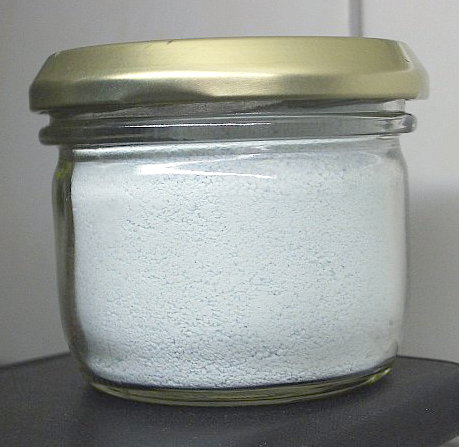
\includegraphics[width=\linewidth,height=4.2cm,keepaspectratio]{images/book1/cuso4-anhydrous.jpg}

{\small Watervrij kopersulfaat: een wit poeder. Foto: W.~Oelen,
CC BY-SA 3.0.}
\end{minipage}\hfill
\begin{minipage}[b]{0.48\linewidth}\centering
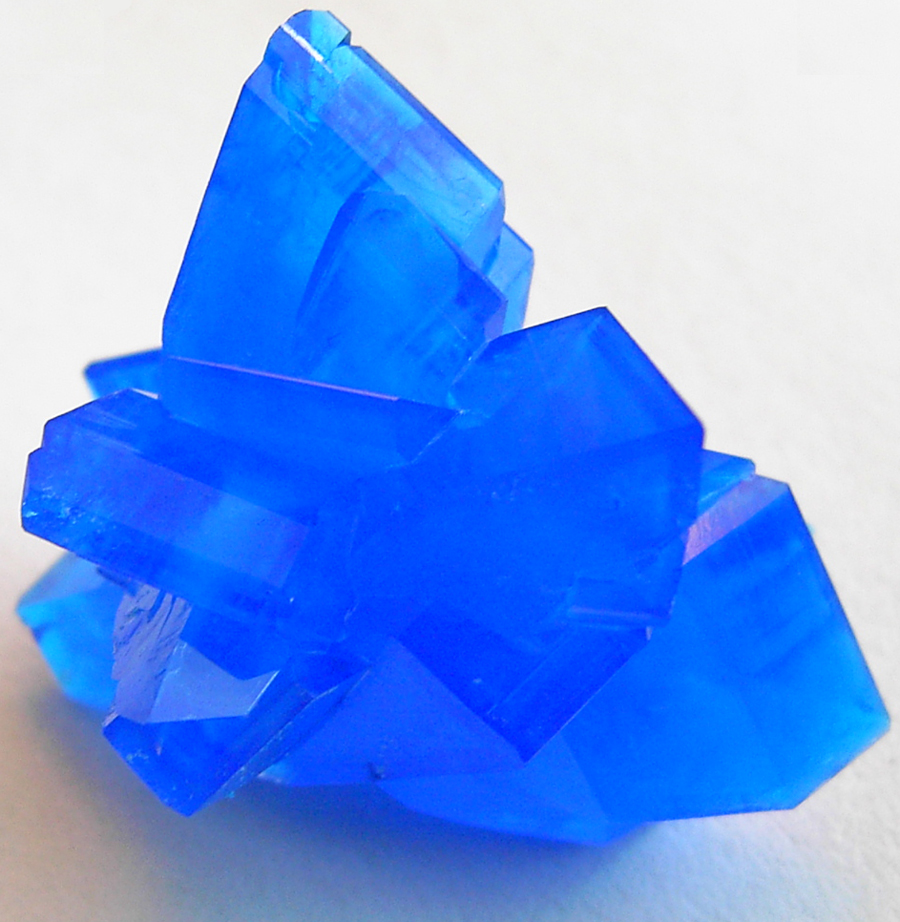
\includegraphics[width=\linewidth,height=4.2cm,keepaspectratio]{images/book1/cuso4-hydrated.jpg}

{\small Met water wordt het blauw; deze kristallen bevatten water. Foto:
Stephanb, CC BY-SA 3.0.}
\end{minipage}
\end{omfigure}

\begin{safety}{\ghs[0.82cm]{GHS05}\ghs[0.82cm]{GHS07}\ghs[0.82cm]{GHS09}}
% ledger: ghs:CuSO4
Kopersulfaat: schadelijk bij inslikken en irriterend voor de huid
(GHS07); het kan ernstig oogletsel veroorzaken (GHS05); zeer giftig voor
in het water levende organismen, met langdurige gevolgen (GHS09).
Veiligheidsbril en handschoenen; het afval wordt ingezameld, nooit door
de gootsteen gespoeld.
\end{safety}

\begin{proposition}[Zuurstof doet een gloeiende houtspaander weer opvlammen]\label{prop:g7:identifying-substances:splint}
Een houten spaander wordt aangestoken en daarna uitgeblazen, zodat er
alleen nog een rode gloed over is. Steek je de gloeiende spaander in een
reageerbuis met zuurstof, dan vlamt hij weer op.
\end{proposition}

\begin{proposition}[Waterstof verbrandt met een blaffend plofje]\label{prop:g7:identifying-substances:pop}
Een brandende spaander bij de opening van een kleine reageerbuis met
waterstof geeft een kort, blaffend ``plofje'': de waterstof verbrandt in
één keer met de zuurstof van de \omterm{def:g4:air-a-mixture-of-gases:air}{lucht}.
\end{proposition}

\begin{omfigure}
\begin{tikzpicture}[font=\small, scale=1.25]
  % splint test for oxygen
  \pic[transform shape] at (0,0) {testtube={0}{white}};
  \draw[brown!60!black, line width=2pt] (0.15,1.6) -- (1.4,3.6);
  \fill[orange!85] (0.15,1.6) circle (0.07);
  \fill[orange!80] (0.12,1.62) .. controls (0.0,1.9) and (0.08,2.1) .. (0.1,2.3)
    .. controls (0.2,2.05) and (0.3,1.85) .. (0.2,1.62);
  \node[anchor=north, align=center] at (0,-0.15) {zuurstof:\\ de gloeiende spaander\\ vlamt op};
  % pop test for hydrogen
  \begin{scope}[xshift=4cm]
    \pic[transform shape, rotate=180] at (0,3.1) {testtube={0}{white}};
    \draw[brown!60!black, line width=2pt] (0.05,-0.05) -- (1.3,-0.9);
    \fill[orange!85] (0.05,-0.02) .. controls (-0.05,0.08) and (0.0,0.15) .. (0.02,0.22)
      .. controls (0.08,0.15) and (0.15,0.08) .. (0.1,-0.02);
    \node[font=\small\itshape] at (-0.9,0.15) {plof!};
    \node[anchor=north, align=center] at (0,-1.0) {waterstof:\\ een blaffend plofje\\ bij de opening};
  \end{scope}
\end{tikzpicture}

{\small Links: een gloeiende spaander vlamt weer op in zuurstof. Rechts:
een brandende spaander bij de opening van een omgekeerde buis met
waterstof geeft een blaffend plofje (waterstof is lichter dan \omterm{def:g4:air-a-mixture-of-gases:air}{lucht},
dus de buis wordt met de opening naar beneden gehouden).}
\end{omfigure}

\begin{safety}{\ghs[0.82cm]{GHS02}\ghs[0.82cm]{GHS04}}
% ledger: ghs:H2
Waterstof: zeer licht ontvlambaar gas (GHS02), onder druk opgeslagen in
gasflessen (GHS04). De knalgasproef wordt met maar een paar milliliter
gedaan, door de docent.
\end{safety}

\section{Papierchromatografie}

\begin{definition}[Papierchromatografie en chromatogram]\label{def:g7:identifying-substances:chromatography}
\emph{Papierchromatografie}\index{papierchromatografie} scheidt de
kleurstoffen van een \omterm{def:g6:pure-substances-and-mixtures:mixture}{mengsel}. Je zet een kleine stip van het \omterm{def:g6:pure-substances-and-mixtures:mixture}{mengsel} op
een lijn die vlak boven de onderkant van een strook papier getekend is;
de onderkant van de strook staat in een \omterm{def:g6:solutions-and-solubility:solute}{oplosmiddel}, dat langzaam in het
papier omhoogkruipt en elke kleurstof meeneemt, de ene sneller dan de
andere. Als het \omterm{def:g6:solutions-and-solubility:solute}{oplosmiddel} bijna bovenaan is, haal je de strook eruit en
laat je haar drogen: dat is het
\emph{chromatogram}\index{chromatogram}.
\end{definition}

\begin{omfigure}
\begin{tikzpicture}[font=\small, scale=1.3]
  % the strip in a beaker of solvent
  \pic[transform shape] at (0,0) {beaker={0.12}{omWater!80}};
  \fill[white] (-0.42,0.06) rectangle (0.42,2.2);
  \fill[omWater!80] (-0.42,0.06) rectangle (0.42,0.24);
  \draw[omGlass, line width=0.6pt] (-0.42,0.06) rectangle (0.42,2.2);
  \draw[black!60, line width=0.4pt] (-0.42,0.42) -- (0.42,0.42);
  \fill[black!80] (0,0.42) circle (0.07);
  \shade[ball color=black!20] (0,2.27) circle (0.08);
  \draw[black!50, line width=1.2pt] (-1.1,2.27) -- (1.1,2.27);
  \node[anchor=north, align=center] at (0,-0.15) {bij de start};
  \draw[<-, omProp, thick] (0.1,0.5) -- (1.3,0.8) node[right, text=black]
    {inktstip op een potloodlijn};
  \draw[<-, omProp, thick] (1.0,2.27) -- (1.3,2.5) node[right, text=black]
    {glazen staaf met het papier};
  \draw[<-, omProp, thick] (0.75,0.15) -- (1.3,0.25) node[right, text=black]
    {oplosmiddel, onder de lijn};
  % the chromatogram
  \begin{scope}[xshift=6.2cm]
    \pic[transform shape] at (0,0) {tlcplate};
    \draw[black!50, dashed] (-0.7,2.7) -- (0.7,2.7);
    \fill[blue!70] (0,1.0) ellipse (0.13 and 0.09);
    \fill[red!70] (0,1.7) ellipse (0.13 and 0.09);
    \fill[yellow!80!orange] (0,2.35) ellipse (0.13 and 0.09);
    \node[anchor=north, align=center] at (0,-0.15) {het chromatogram};
    \draw[<-, omProp, thick] (0.75,2.7) -- (1.3,2.85) node[right, text=black]
      {hoe ver het oplosmiddel kwam};
    \draw[<-, omProp, thick] (0.2,1.7) -- (1.3,1.7) node[right, text=black]
      {drie kleurstoffen: een mengsel};
  \end{scope}
\end{tikzpicture}

{\small \omterm{def:g7:identifying-substances:chromatography}{Papierchromatografie} van een zwarte inkt. Het \omterm{def:g6:solutions-and-solubility:solute}{oplosmiddel} kruipt
omhoog door het papier en scheidt de inkt in drie kleurstoffen.}
\end{omfigure}

\begin{method}[Een chromatogram lezen]\label{met:g7:identifying-substances:read}
\begin{enumerate}
  \item Tel de vlekken boven elk startpunt: één vlek, één kleurstof; twee
        vlekken of meer, een \omterm{def:g6:pure-substances-and-mixtures:mixture}{mengsel} van kleurstoffen.
  \item Vergelijk de hoogtes: in hetzelfde \omterm{def:g7:identifying-substances:chromatography}{chromatogram} komt een
        kleurstof altijd even hoog. Een vlek op dezelfde hoogte als een
        bekende kleurstof is waarschijnlijk die kleurstof.
  \item Gebruik een potloodlijn, nooit inkt: inkt zou zelf door het
        \omterm{def:g6:solutions-and-solubility:solute}{oplosmiddel} gescheiden worden.
\end{enumerate}
\end{method}

\begin{example}[De kleurstoffen van snoepjes]\label{ex:g7:identifying-substances:sweets}
Het gekleurde laagje van snoepjes wordt in een beetje water afgeschraapt
en op een strook gestipt, naast stippen van de voedingskleurstoffen die
in snoep zijn toegestaan. Het \omterm{def:g7:identifying-substances:chromatography}{chromatogram} laat zien dat het groene
laagje een gele en een blauwe kleurstof bevat, die allebei bij de
toegestane kleurstoffen horen.
\end{example}


\section{Een testoverzicht lezen}

\begin{proposition}[Een tabel van aantoningsreacties]\label{prop:g7:identifying-substances:bank}
Scheikundigen zetten de tests die ze gebruiken in een tabel, een
testoverzicht, dat je van links naar rechts leest:
\begin{center}
\small
\begin{tabular}{llll}
\hline
gezochte stof & \omterm{def:g7:identifying-substances:characteristic-test}{reagens} of test & positief resultaat & \\
\hline
koolstofdioxide & kalkwater & kalkwater wordt troebel & \\
water & watervrij kopersulfaat & wit wordt blauw & \\
zuurstof & gloeiende spaander & de spaander vlamt op & \\
waterstof & brandende spaander & een blaffend plofje & \\
kleurstoffen van een \omterm{def:g6:pure-substances-and-mixtures:mixture}{mengsel} & \omterm{def:g7:identifying-substances:chromatography}{papierchromatografie} & één vlek per kleurstof & \\
\hline
\end{tabular}
\end{center}
\end{proposition}

\begin{remark}[Wat een test niet zegt]\label{rem:g7:identifying-substances:limits}
Een positieve test bewijst dat de stof aanwezig is, niet dat ze alleen
is: een vloeistof die kopersulfaat blauw kleurt, bevat water, maar het
kan zout water of sinaasappelsap zijn. Een negatieve test zegt alleen dat
de stof afwezig is, of aanwezig in een te kleine hoeveelheid om iets te
laten zien.
\end{remark}

\begin{omfigure}
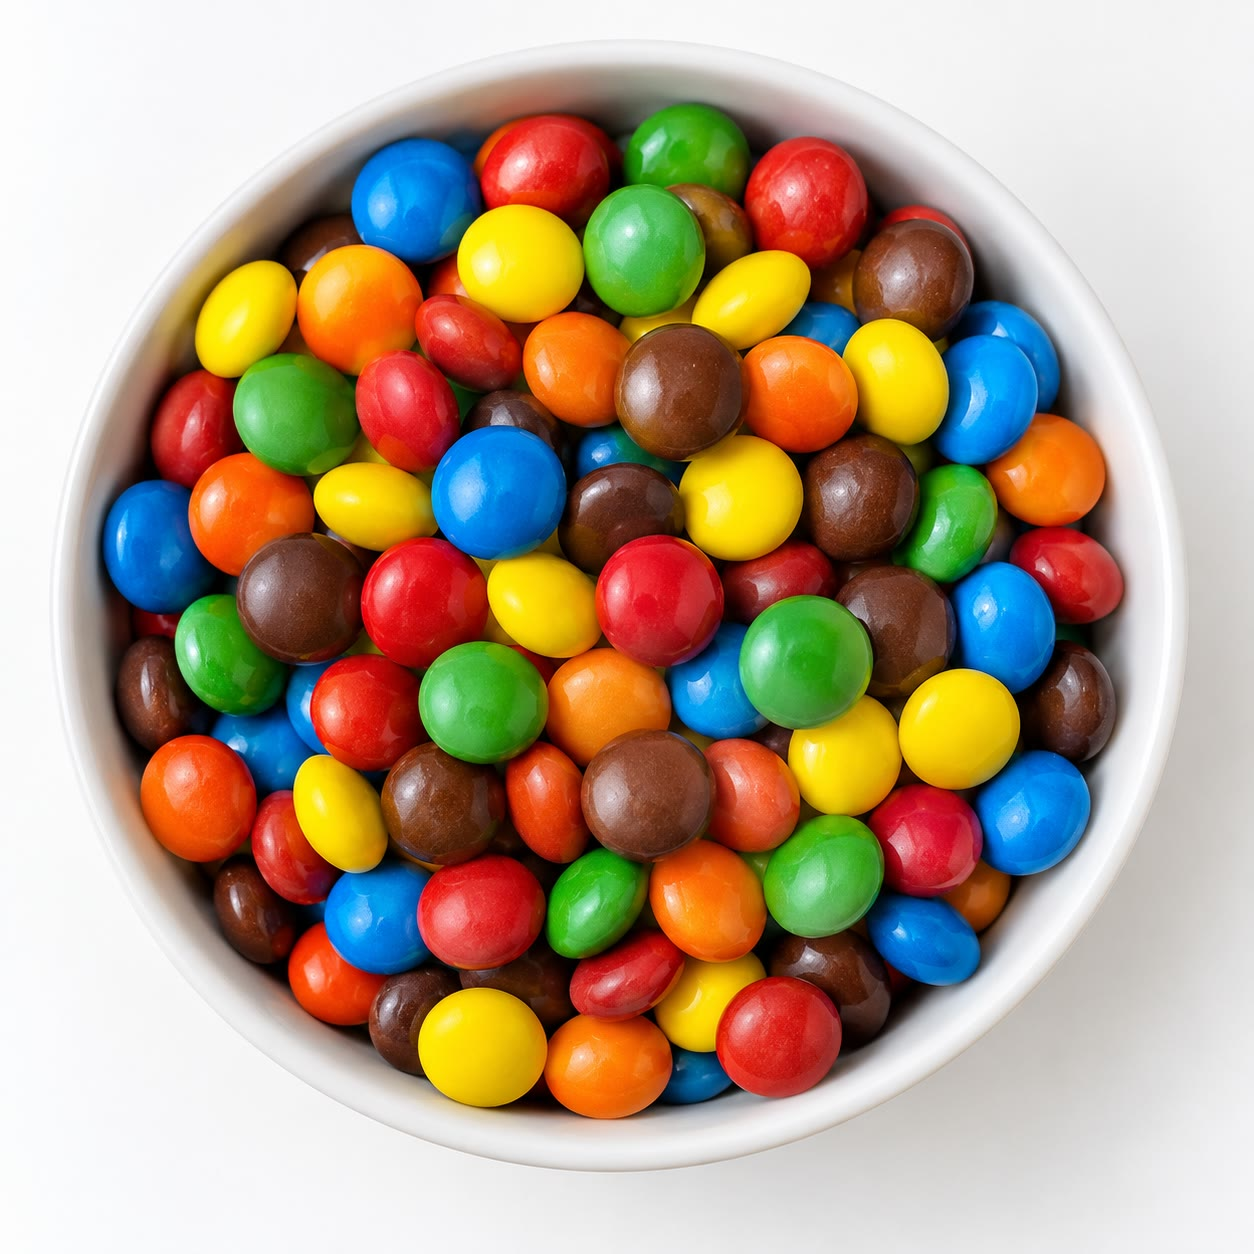
\includegraphics[width=0.32\linewidth]{images/book1/ai/g7-sweets.jpg}

{\small Snoepjes met een suikerlaagje: hun kleuren zijn \omterm{def:g6:pure-substances-and-mixtures:mixture}{mengsels} van
kleurstoffen die chromatografie kan scheiden.}
\end{omfigure}

\begin{omfigure}
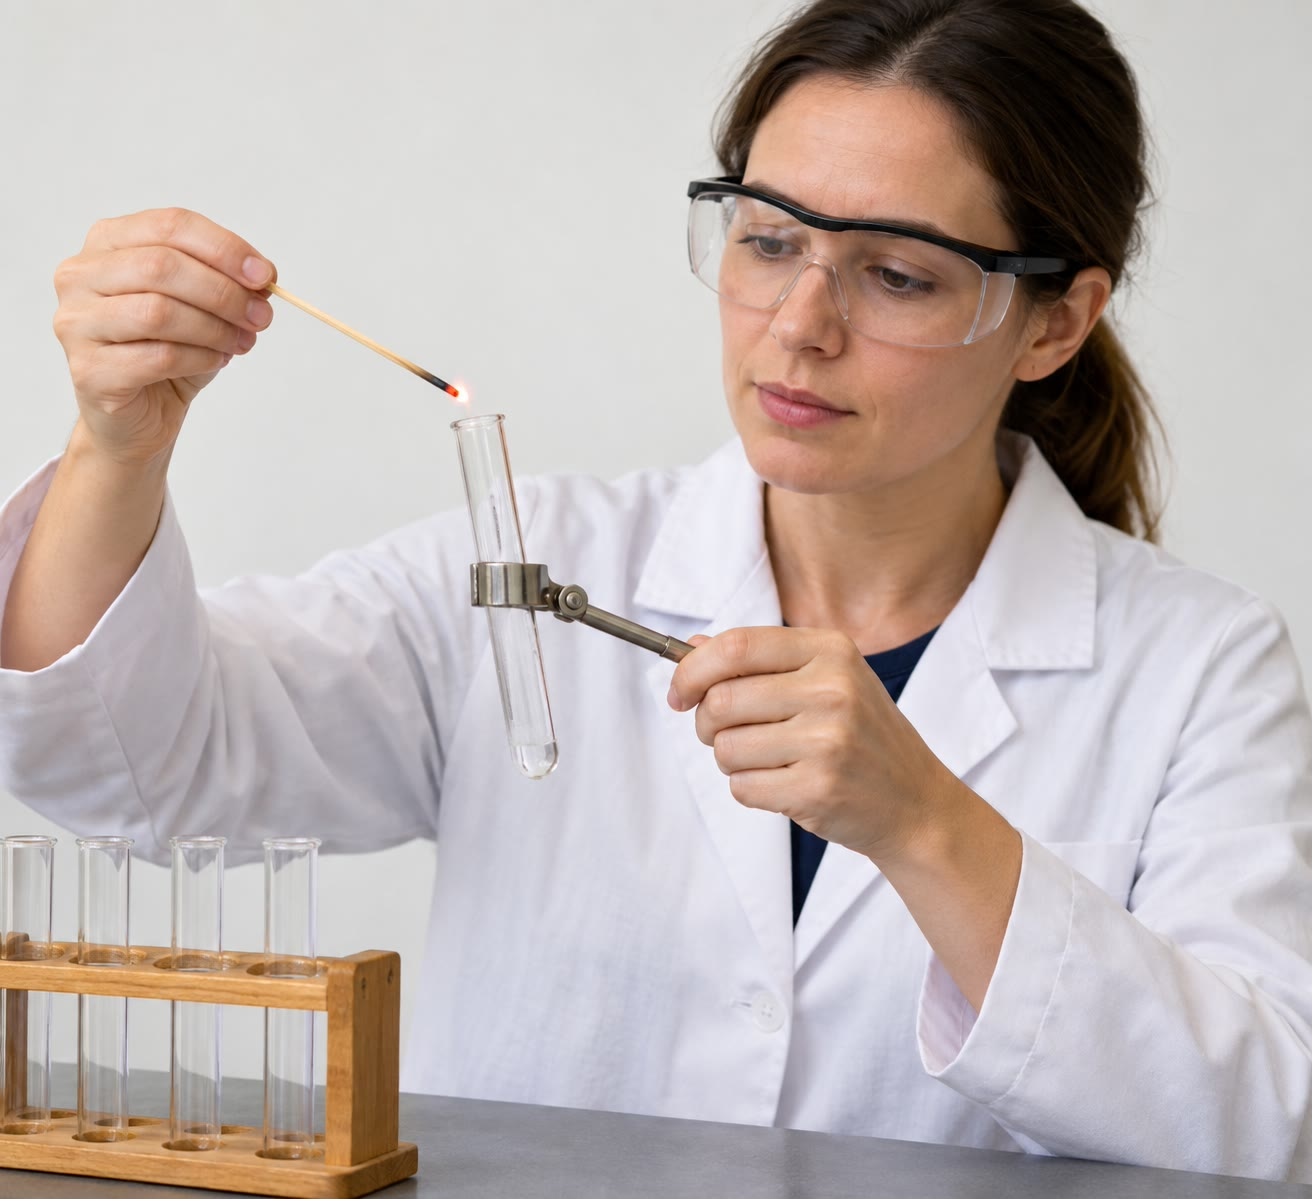
\includegraphics[width=0.36\linewidth]{images/book1/ai/g7-splint-teacher.jpg}

{\small Een docent test een gas met een gloeiende spaander.}
\end{omfigure}

\section{Oefeningen}

\begin{exercise}[$\star$]\label{exo:g7:identifying-substances:1}
Met welke test toon je koolstofdioxide aan? Beschrijf het positieve
resultaat.
\end{exercise}

\begin{exercise}[$\star$]\label{exo:g7:identifying-substances:2}
Een wit poeder wordt blauw als er een vloeistof op gedruppeld wordt. Wat
laat dat zien over de vloeistof?
\end{exercise}

\begin{exercise}[$\star$]\label{exo:g7:identifying-substances:3}
Een gloeiende spaander wordt in een gaspot gestoken en vlamt op. Welk gas
zit er in de pot?
\end{exercise}

\begin{exercise}[$\star$]\label{exo:g7:identifying-substances:4}
Waarom teken je de startlijn van een papierchromatogram met potlood en
niet met inkt?
\end{exercise}

\begin{exercise}[$\star\star$]\label{exo:g7:identifying-substances:5}
Waarom moet de startlijn boven het niveau van het \omterm{def:g6:solutions-and-solubility:solute}{oplosmiddel} in het
bekerglas liggen?
\end{exercise}

\begin{exercise}[$\star\star$]\label{exo:g7:identifying-substances:6}
Een \omterm{def:g7:identifying-substances:chromatography}{chromatogram} van een groene inkt laat twee vlekken zien, een op de
hoogte van een gele referentiekleurstof en een op de hoogte van een
blauwe referentiekleurstof. Is de groene inkt een \omterm{def:g6:pure-substances-and-mixtures:pure-substance}{zuivere stof}? Waaruit
bestaat hij?
\end{exercise}

\begin{exercise}[$\star\star$]\label{exo:g7:identifying-substances:7}
Welke test uit het testoverzicht zou je gebruiken om te laten zien dat
een gas dat bij een reactie ontstaat waterstof is? Wat verwacht je te
zien?
\end{exercise}

\begin{exercise}[$\star\star$]\label{exo:g7:identifying-substances:8}
Uitgeademde \omterm{def:g4:air-a-mixture-of-gases:air}{lucht} maakt kalkwater veel sneller troebel dan frisse \omterm{def:g4:air-a-mixture-of-gases:air}{lucht}.
Wat vertelt dat ons over de \omterm{def:g4:air-a-mixture-of-gases:air}{lucht} die we uitademen?
\end{exercise}

\begin{exercise}[$\star\star$]\label{exo:g7:identifying-substances:9}
Een heldere vloeistof kleurt watervrij kopersulfaat blauw. Sam
concludeert: ``Het is zuiver water.'' Leg uit waarom Sam ongelijk heeft.
\end{exercise}

\begin{exercise}[$\star\star$]\label{exo:g7:identifying-substances:10}
Kijk naar het \omterm{def:g7:identifying-substances:chromatography}{chromatogram} van de zwarte inkt in dit hoofdstuk. Hoeveel
kleurstoffen bevat de inkt? Welke is het hoogst gekomen?
\end{exercise}

\begin{exercise}[$\star\star\star$]\label{exo:g7:identifying-substances:11}
Drie potten bevatten zuurstof, waterstof en koolstofdioxide, maar hun
etiketten zijn kwijt. Plan op papier de tests waarmee je elke pot een
naam geeft, in een volgorde die zo weinig mogelijk tests gebruikt.
\end{exercise}

\begin{exercise}[$\star\star\star$]\label{exo:g7:identifying-substances:12}
Een leerling test een gas met kalkwater en ziet niets gebeuren. Geef twee
mogelijke verklaringen, en de controleproef die zou helpen kiezen.
\end{exercise}

\section{Probleem: Het vervalste briefje}

\begin{problem}[{Weekendprobleem --- een briefje in viltstift, drie
verdachte stiften, drie gasflessen zonder etiket, en een testoverzicht}]
\label{pb:g7:identifying-substances:1}
Het schoollaboratorium wordt gevraagd te helpen bij twee kleine
mysteries. Eerst moet een briefje dat met zwarte viltstift geschreven is,
gekoppeld worden aan een van drie zwarte stiften, 1, 2 en 3. Van het
briefje en van elke stift wordt een druppel inkt genomen en op dezelfde
strook papier gestipt, die daarna met water wordt ontwikkeld. Het
\omterm{def:g7:identifying-substances:chromatography}{chromatogram} staat hieronder.
\begin{center}
\begin{tikzpicture}[font=\small, x=1cm, y=1cm]
  \fill[white] (0,0) rectangle (6,4);
  \draw[omGlass, line width=0.6pt] (0,0) rectangle (6,4);
  \draw[black!60] (0,0.5) -- (6,0.5);
  \draw[black!50, dashed] (0,3.6) -- (6,3.6);
  \foreach \x/\lab in {0.9/briefje, 2.3/stift 1, 3.7/stift 2, 5.1/stift 3}
    \node[anchor=north] at (\x,-0.05) {\lab};
  % note: three dyes
  \fill[blue!70] (0.9,1.2) ellipse (0.18 and 0.1);
  \fill[red!70] (0.9,2.2) ellipse (0.18 and 0.1);
  \fill[yellow!80!orange] (0.9,3.1) ellipse (0.18 and 0.1);
  % pen 1: two dyes
  \fill[blue!70] (2.3,1.2) ellipse (0.18 and 0.1);
  \fill[black!70] (2.3,2.7) ellipse (0.18 and 0.1);
  % pen 2: same three as the note
  \fill[blue!70] (3.7,1.2) ellipse (0.18 and 0.1);
  \fill[red!70] (3.7,2.2) ellipse (0.18 and 0.1);
  \fill[yellow!80!orange] (3.7,3.1) ellipse (0.18 and 0.1);
  % pen 3: three dyes, other heights
  \fill[violet!70] (5.1,0.9) ellipse (0.18 and 0.1);
  \fill[red!70] (5.1,1.8) ellipse (0.18 and 0.1);
  \fill[green!60!black] (5.1,2.6) ellipse (0.18 and 0.1);
  \node[anchor=west, font=\footnotesize] at (6.1,3.6) {front van het oplosmiddel};
  \node[anchor=west, font=\footnotesize] at (6.1,0.5) {startlijn};
\end{tikzpicture}
\end{center}

\medskip
\noindent\textbf{Deel I --- Het \omterm{def:g7:identifying-substances:chromatography}{chromatogram}.}
\begin{enumerate}
  \item Waarom zijn alle vier de inkten op dezelfde strook gestipt en
        samen ontwikkeld?
  \item Is de inkt van het briefje een \omterm{def:g6:pure-substances-and-mixtures:pure-substance}{zuivere stof} of een \omterm{def:g6:pure-substances-and-mixtures:mixture}{mengsel}? Leg
        uit.
  \item Hoeveel kleurstoffen bevat de inkt van stift 1? Kan stift 1 het
        briefje geschreven hebben?
  \item Stift 3 bevat ook drie kleurstoffen. Waarom kan die het briefje
        niet geschreven hebben?
  \item Welke stift past bij het briefje? Leg uit met de hoogtes van de
        vlekken.
\end{enumerate}

\medskip
\noindent\textbf{Deel II --- Drie gasflessen.}
Het tweede mysterie: drie kleine gasflessen, X, Y en Z, zijn hun etiket
kwijt; ze bevatten zuurstof, waterstof en koolstofdioxide. Van elke fles
wordt een beetje gas in een reageerbuis opgevangen. Gas X doet een
gloeiende spaander weer opvlammen. Gas Y geeft met een brandende
spaander een blaffend plofje. Gas Z maakt kalkwater troebel.
\begin{enumerate}[resume]
  \item Geef de naam van gas X.
  \item Geef de naam van gas Y.
  \item Geef de naam van gas Z.
  \item Voordat de leerling gas Z test, leidt ze gewone \omterm{def:g4:air-a-mixture-of-gases:air}{lucht} even lang
        door hetzelfde kalkwater, en dat blijft helder. Hoe heet deze
        tweede proef, en wat voegt ze toe aan de conclusie?
\end{enumerate}

\medskip
\noindent\textbf{Deel III --- Het testoverzicht.}
\begin{enumerate}[resume]
  \item Een kleurloze vloeistof die naast het briefje gevonden is, kleurt
        watervrij kopersulfaat blauw. Schrijf de regel van het
        testoverzicht op die je gebruikt, en wat het resultaat laat zien.
  \item Bewijst dit resultaat dat de vloeistof zuiver water is? Leg uit.
  \item Sluit het eerste mysterie af: hoeveel kleurstoffen bevat de inkt
        van het briefje, en welke stift heeft het geschreven?
\end{enumerate}
\end{problem}
